\documentclass[conference]{IEEEtran}
\usepackage[british]{babel}
\usepackage[T1]{fontenc}
\usepackage{amsmath,amssymb,bm}
\usepackage{booktabs}
\usepackage{array}
\usepackage{cite}
\usepackage{graphicx}
\usepackage{url}
\usepackage{algorithm}
\usepackage{algorithmic}
\usepackage{flafter}
\usepackage[caption=false,font=normalsize]{subfig}

\newcommand{\knn}{\mbox{$k$-NN}}
\renewcommand{\algorithmicforall}{\textbf{for each}}

\begin{document}
\raggedbottom
\title{Neural Network Ensembles and Stacking for Network Traffic Classification}
\author{\IEEEauthorblockN{Student number: 27233162}}
\maketitle

\begin{abstract}
    Ensemble learning was investigated on 257\,673 network connection records to test whether dissimilar classifiers improve intrusion classification. A weight-sharing neural network ensemble, TabM, was evaluated alone and within a stack combining the re-tuned nearest neighbour and decision tree models of an earlier study. The comparison reused the earlier grouped five-fold evaluation, with nine questions guiding tuning and per-class analysis. The three-learner stack had the highest macro F-score, $0.603 \pm 0.010$, against $0.575 \pm 0.017$ for the earlier tree, and scored higher on every fold. The difference was not significant under the corrected test, with $p = 0.076$. TabM alone scored 0.525, yet improved the stack on every fold, consistent with complementary errors between TabM and the class-weighted tree. The revised tree recovered more minority attacks, whereas TabM classified frequent classes more accurately. Learned stacking combined these different precision--recall trade-offs, although equal-weight averaging remained competitive and no ensemble improved every attack class. Class weights, distinct minibatches and dropout lowered the TabM tuning score. The findings applied to one dataset and a protocol revised after the first test results were known.

\end{abstract}

\begin{IEEEkeywords}
    ensemble learning, stacked generalisation, neural networks, intrusion classification
\end{IEEEkeywords}

\section{Introduction}
The strongest individual classifier need not supply every useful prediction for an ensemble. An earlier study of network intrusion classification found that a decision tree outperformed $k$-nearest neighbours (\knn) in macro F-score. However, \knn{} performed better on denial of service (DoS) and Analysis. These class-specific differences motivated a comparison of models with different inductive biases, the assumptions about the input--output relationship that guide learning \cite{dietterich2000}.

The present study compared TabM and stacked generalisation with the earlier models. TabM combines multilayer perceptrons (MLPs) through shared weight matrices\cite{gorishniy2025}. Stacked generalisation, or stacking, trains a meta-learner on predictions from several base learners \cite{wolpert1992}. A random forest or boosted trees would instead extend the partitioning rules of the earlier tree to address bias or variance\cite{hastie2009}. The chosen comparison asked whether a neural learner supplied useful information beyond the local neighbourhoods of \knn{} and the feature-specific splits of a tree.

The research question was whether either ensemble improved macro F-score on the same outer folds, and what the tuning revealed about the differences. Nine questions addressed ensemble size, weighting, member diversity, capacity, the learned combination and class-specific performance. Reproducing and re-tuning the earlier models provided the original baselines and stronger individual learners for the ensemble comparison.

Stacking had the highest mean macro F-score, but the comparison did not establish a significant gain over the earlier tree. A weaker TabM improved the stack on every fold, showing that standalone ranking did not describe the usefulness of a base learner. Section~II gives the model background. Sections~III and IV describe the implementation and empirical process. Section~V interprets the results, and Section~VI concludes the report.

\section{Background}
This section describes the classification task and the two models of the earlier study. The section then covers the principles of ensemble learning, the two ensembles and the tests for comparing models over cross-validation folds.

\subsection{Network Intrusion Classification}
Network intrusion classification assigns a connection record to normal traffic or an attack category. The input consists of recorded flow statistics, such as byte counts, packet rates, duration and protocol. The task therefore concerns classification from summarised connection attributes rather than from the original packet contents \cite{moustafa2015}.

\subsection{Nearest Neighbour Classification}
Nearest neighbour classification predicts the label of a query observation from the labels of the most similar training observations \cite{cover1967}. The method stores the $n$ training pairs $(\mathbf{x}_i, y_i)$ and fits no parameters. The method rests on the assumption that observations close together in the feature space tend to belong to the same class. A distance function makes closeness measurable. The function reduces all feature differences between two observations to one non-negative number, and identical observations have distance zero. The choice of distance function therefore determines the training observations that decide each prediction.

For two vectors $\mathbf{x}$ and $\mathbf{x}'$ with $m$ features, the Minkowski distance of order $q$ is
\begin{equation}
    d(\mathbf{x},\mathbf{x}') = \Big(\sum_{j=1}^{m} |x_j - x'_j|^{q}\Big)^{1/q},
\end{equation}
where $x_j$ is feature $j$ of $\mathbf{x}$. The order $q=1$ gives the Manhattan distance, the sum of the absolute differences along the feature axes. The order $q=2$ gives the Euclidean distance, the straight-line length between two points. The Manhattan distance counts every unit of difference equally, whatever the feature. The Euclidean distance squares the differences, so one large difference counts for more than several small differences with the same sum. A larger order gives still more weight to the largest single difference.

Every feature enters the sum on the numerical scale of the feature, so a feature with a range of millions dominates a feature with a range of one. Numeric features are therefore rescaled to comparable ranges before distances are computed \cite{hastie2009}. Every feature also counts in the distance, whether or not the feature carries class information. Irrelevant features add variation to every distance and so blur the contrast between near and distant observations. In many dimensions, a neighbourhood must also span a large part of the range of every feature to contain a fixed share of the training observations. The nearest observations are then no longer local \cite{hastie2009}.

Nominal features have no numerical order. One-hot encoding replaces a nominal feature with one binary indicator for each level. Two observations with different levels then differ in two indicators, and the Manhattan distance between the observations grows by two. Every pair of distinct levels therefore contributes the same amount to the distance.

To classify a query observation $\mathbf{x}$, the method finds the index set $N_k(\mathbf{x})$ of the $k$ training observations nearest to $\mathbf{x}$. Each neighbour $i$ casts a vote with weight $w_i$ for the class $y_i$. The estimated probability of class $l$ is the weighted share of the votes,
\begin{equation}
    \hat{\pi}_l(\mathbf{x}) = \frac{\sum_{i\in N_k(\mathbf{x})} w_i\,\delta(y_i,l)}{\sum_{i\in N_k(\mathbf{x})} w_i},
\end{equation}
where $\delta(y_i,l)$ is one when $y_i=l$ and zero otherwise. The predicted class $\hat{y}$ is the class with the largest estimated probability. Uniform weighting sets $w_i=1$. Distance weighting sets $w_i = 1/d(\mathbf{x},\mathbf{x}_i)$, so closer neighbours count more. If a neighbour has zero distance, only zero-distance neighbours vote. With $k=3$ and uniform weights, every probability is a multiple of one third, so the estimates are coarse. Algorithm~\ref{alg:knn} summarises the classification of one query observation.

\begin{algorithm}[!t]
    \caption{Nearest neighbour classification of one query observation}
    \label{alg:knn}
    \begin{algorithmic}[1]
        \STATE Store the $n$ training observations and labels.
        \FORALL{training observation $i$}
        \STATE Compute the distance $d(\mathbf{x},\mathbf{x}_i)$ to the query observation $\mathbf{x}$.
        \ENDFOR
        \STATE Form $N_k(\mathbf{x})$ from the $k$ observations with the smallest distances.
        \STATE Give each neighbour $i$ the vote weight $w_i$.
        \STATE Estimate $\hat{\pi}_l(\mathbf{x})$ for each class $l$ from the weighted votes.
        \STATE Predict the class with the largest estimated probability.
    \end{algorithmic}
\end{algorithm}

The number of neighbours $k$ controls a trade-off between bias and variance \cite{hastie2009}. With $k=1$, the nearest training observation alone decides the prediction. Every query observation whose nearest neighbour is mislabelled then receives the wrong class. With a larger $k$, a mislabelled neighbour supplies one of $k$ votes and changes the prediction only when the other neighbours split their votes. A larger $k$ therefore averages out label noise and isolated atypical observations, and the boundaries between class regions become smoother.

The cost of a larger $k$ is bias, because a large neighbourhood reaches into the regions of other classes. A neighbourhood larger than the cluster of a rare class necessarily contains observations of other classes, so frequent classes nearby compete with the rare class in every vote. Distance weighting reduces the bias, because nearer neighbours count more. Under distance weighting, a mislabelled observation very close to the query also keeps a large weight. The neighbourhood is ambiguous when several training observations lie at exactly the distance of the $k$-th neighbour. Any subset of the tied observations completes a valid neighbourhood, and different implementations choose different subsets.

\subsection{Decision Tree Classification}
A classification tree partitions the feature space with a sequence of binary tests \cite{breiman1984}. Each internal node tests one feature against a threshold, $x_j \le \theta$, and sends an observation to the left or the right child. Each leaf stores the class proportions of the training observations that reach the leaf. A query observation follows the tests from the root to a leaf. The tree predicts the most frequent class of the leaf, and the leaf proportions serve as class probability estimates.

Growing the tree selects, at each node $t$, the test that makes the child nodes as pure as possible. Impurity measures how mixed the classes are among the training observations $S_t$ at node $t$. Impurity is zero when all observations at the node share one class, and maximal when all $K$ classes are equally frequent. Let $\pi_l(t)$ be the proportion of class $l$ among the observations in $S_t$. The Gini impurity
\begin{equation}
    G(t) = 1 - \sum_{l=1}^{K} \pi_l(t)^2
\end{equation}
is the probability that two observations drawn at random with replacement from $S_t$ belong to different classes. The entropy
\begin{equation}
    H(t) = -\sum_{l=1}^{K} \pi_l(t) \log_2 \pi_l(t)
\end{equation}
is the average information content, in bits, of the class of an observation drawn from $S_t$ \cite{hastie2009}. A test sends the observations $S_L$ to the left child $t_L$ and the observations $S_R$ to the right child $t_R$. For unweighted observations and impurity $Q$ equal to $G$ or $H$, the impurity decrease is
\begin{equation}
    \Delta Q = Q(t) - \frac{|S_L|}{|S_t|}Q(t_L) - \frac{|S_R|}{|S_t|}Q(t_R).
\end{equation}
The algorithm evaluates every candidate feature and threshold, applies the test with the largest decrease and repeats the search in each child.

Impurity matters because the impurity decrease chooses the test at every node, and each chosen test constrains all descendant nodes. A pure leaf predicts one class with probability one, whereas an impure leaf gives graded probabilities. The misclassification rate of a node would be a simpler criterion, but the rate fails to separate many candidate tests. Hastie \emph{et al.} illustrated the problem with 400 observations of each of two classes \cite{hastie2009}. A split into nodes with class counts $(300,100)$ and $(100,300)$ misclassified 200 observations, as did a split into nodes with counts $(200,400)$ and $(200,0)$. Only the second split created a pure node, and both the Gini impurity and the entropy were lower for the second split. Impurity therefore rewards progress towards pure nodes that the misclassification rate ignores. No test separates observations with identical feature values, so a node that holds identical observations with different labels keeps a positive impurity at any depth.

Unrestricted growth fits increasingly specific patterns in the training observations, including label noise. Maximum depth and minimum node sizes limit growth. Cost-complexity pruning balances fit against the number of leaves \cite{breiman1984}. The implemented tree minimises $e(T) + \alpha|T|$, where $e(T)$ is the total sample-weighted leaf impurity, $|T|$ counts the leaves and $\alpha \ge 0$ penalises each leaf. Scikit-learn uses impurity rather than the misclassification rate of the classical formulation. Algorithm~\ref{alg:tree} summarises the growth and pruning of a tree.

\begin{algorithm}[!t]
    \caption{Growth and pruning of a classification tree}
    \label{alg:tree}
    \begin{algorithmic}[1]
        \STATE Place all training observations in the root node.
        \FORALL{node $t$, in the order of creation}
        \IF{$t$ is pure, has the maximum depth, holds fewer observations than the minimum split size or allows no valid test}
        \STATE Make $t$ a leaf that stores the class proportions $\pi_l(t)$.
        \ELSE
        \STATE Compute $\Delta Q$ for every candidate feature $j$ and threshold $\theta$.
        \STATE Apply the test $x_j \le \theta$ with the largest $\Delta Q$ among the tests that leave at least the minimum leaf size in each child.
        \STATE Add the two child nodes.
        \ENDIF
        \ENDFOR
        \STATE Prune the tree to the subtree $T$ that minimises $e(T) + \alpha|T|$.
    \end{algorithmic}
\end{algorithm}

Class weights $\omega_l$ multiply the contribution of each training observation of class $l$. Balanced weights $\omega_l = n/(K n_l)$, where $n_l$ counts training observations of class $l$, give every class the same total weight $n/K$. The weights affect class proportions, impurity, split selection and pruning. Child-size ratios in the impurity decrease then use total weights rather than observation counts. Weighting therefore changes both the partition and the leaf predictions. A tree depends on feature order rather than numerical scale, but small changes to the data can change the selected splits \cite{hastie2009}.

\subsection{Ensemble Learning}
An ensemble combines the predictions of several models, called members or base learners. Combining members can reduce prediction variance or represent decision boundaries beyond the capacity of one member. Dietterich attributed ensemble benefits to statistical, computational and representational causes \cite{dietterich2000}. Members must make useful predictions and differ in errors for a combination to improve classification. Diversity alone does not guarantee a higher F-score \cite{kuncheva2003}.

Kuncheva and Whitaker compared measures of diversity defined on the errors of pairs of members \cite{kuncheva2003}. The disagreement is the share of observations where two members predict different labels. The double fault is the share of observations that both members misclassify. The error correlation is the correlation between the binary error indicators of two members.

Homogeneous ensembles use one model family. Bagging trains each member on a bootstrap sample and averages the members, mainly reducing prediction variance. Random forests add a random choice of candidate features at each split. In AdaBoost, boosting trains members in sequence and raises the weights of misclassified observations \cite{hastie2009}. Heterogeneous ensembles combine different algorithms, so the members differ in inductive bias even when trained on the same observations \cite{dietterich2000}. The simplest combinations are the majority vote of predicted labels and the soft vote, the average of class probabilities.

\subsection{Stacked Generalisation}
Wolpert introduced stacked generalisation \cite{wolpert1992}. In stacking, a meta-learner learns to combine the predictions of base learners. The meta-features, the inputs of the meta-learner, are the predictions of the base learners for each training observation. The meta-features must come from base learners that did not see the observation. A fully grown tree fits the training observations of the tree almost perfectly, so in-sample meta-features would teach the meta-learner to trust the most overfitted base learner. Stacking therefore obtains out-of-fold meta-features by an internal cross-validation, as Algorithm~\ref{alg:stacking} shows. Each base learner is then refitted on all training observations to produce the meta-features of new observations.

\begin{algorithm}[!t]
    \caption{Stacked generalisation with out-of-fold meta-features}
    \label{alg:stacking}
    \begin{algorithmic}[1]
        \STATE Split the training observations into internal folds.
        \FORALL{internal fold}
        \FORALL{base learner}
        \STATE Fit the base learner on the other internal folds.
        \STATE Predict class probabilities for the held-out fold.
        \ENDFOR
        \ENDFOR
        \STATE Join the probabilities of all base learners into one meta-feature vector for each training observation.
        \STATE Fit the meta-learner on the meta-features and the true labels.
        \STATE Refit every base learner on all training observations.
        \STATE Predict a new observation with the meta-learner from the meta-features that the refitted base learners produce.
    \end{algorithmic}
\end{algorithm}

Ting and Witten found that stacking performed best when the meta-features were class probabilities rather than predicted labels \cite{ting1999}. Probabilities carry the confidence of each base learner, whereas labels discard the confidence. A multinomial logistic regression is a common meta-learner. Let $\mathbf{z}$ be the meta-feature vector of an observation. The model estimates the probability of class $l$ as
\begin{equation}
    \hat{\pi}_l(\mathbf{z}) = \frac{\exp(\bm{\beta}_l^{\mathsf T}\mathbf{z} + \beta_{l,0})}{\sum_{l'=1}^{K}\exp(\bm{\beta}_{l'}^{\mathsf T}\mathbf{z} + \beta_{l',0})},
\end{equation}
with a coefficient vector $\bm{\beta}_l$ and an intercept $\beta_{l,0}$ for each class \cite{hastie2009}. Fitting minimises the penalised negative log-likelihood
\begin{equation}
    \frac{1}{2}\sum_{l=1}^{K}\|\bm{\beta}_l\|^2 - C\sum_{i=1}^{n} \ln\hat{\pi}_{y_i}(\mathbf{z}_i),
\end{equation}
where a smaller inverse regularisation strength $C$ shrinks the coefficients more. An own-class coefficient links the probability of class $l$ from a base learner to the score of class $l$. The final decision depends on all coefficients and all class scores. Coefficient magnitude alone therefore does not measure the importance of a learner. A soft vote averages the base probabilities with equal weights.

\subsection{Multilayer Perceptrons and Weight-Sharing Ensembles}
An MLP maps an input vector through a sequence of layers \cite{goodfellow2016}. Each hidden layer computes $\mathbf{a}' = \max(\mathbf{0}, \mathbf{W}\mathbf{a} + \mathbf{b})$ from the layer input $\mathbf{a}$, with a weight matrix $\mathbf{W}$, a bias vector $\mathbf{b}$ and the elementwise rectified linear unit (ReLU). A final linear layer produces one score for each class, and the softmax function turns the scores into class probabilities. Training minimises the cross-entropy, the mean of $-\ln\hat{\pi}_{y}(\mathbf{x})$ over the training observations, with minibatch gradient steps. The adaptive moment estimation (Adam) optimiser adapts the step size of every weight. Dropout sets randomly chosen hidden units to zero during training and so discourages co-adapted units. Early stopping keeps the weights from the epoch with the best validation score \cite{goodfellow2016}. Adam with decoupled weight decay (AdamW), used in TabM training, applies weight decay separately from the gradient step \cite{gorishniy2025}. On tabular data, tree ensembles outperformed MLPs in a benchmark by Grinsztajn \emph{et al.} \cite{grinsztajn2022}. The authors attributed the gap to the preference of MLPs for smooth functions and to the sensitivity of MLPs to uninformative features.

An ensemble of independently trained networks requires a separate set of weights and a separate fit for every member. BatchEnsemble reduces this cost by sharing one weight matrix $\mathbf{W}$ in each layer among $M$ members \cite{wen2020}. Member $h$ owns two scaling vectors, $\mathbf{r}_h$ and $\mathbf{s}_h$, and a bias vector $\mathbf{b}_h$. For the input $\mathbf{a}_h$ of member $h$, the layer computes the output
\begin{equation}
    \mathbf{o}_h = \mathbf{s}_h \odot \big(\mathbf{W}(\mathbf{r}_h \odot \mathbf{a}_h)\big) + \mathbf{b}_h,
\end{equation}
where $\odot$ is the elementwise product. The output equals the output of an ordinary linear layer with the member weight matrix $\mathbf{W}_h = \mathbf{W} \odot (\mathbf{s}_h\mathbf{r}_h^{\mathsf T})$. Each member therefore uses the shared matrix rescaled by a member-specific matrix of rank one. All members run as one batched matrix product, and each member adds only two vectors and a bias to the shared weights.

TabM uses BatchEnsemble layers in the hidden network and a separate output layer for each member \cite{gorishniy2025}. All members train simultaneously. Training batches are either shared or sampled through separate shuffles for the members. Let $\hat{\pi}_{h,l}(\mathbf{x})$ be the probability that member $h$ assigns to class $l$. The loss for an observation with label $y$ is the mean of the member cross-entropies,
\begin{equation}
    \mathcal{L}(\mathbf{x}, y) = -\frac{1}{M}\sum_{h=1}^{M} \ln \hat{\pi}_{h,y}(\mathbf{x}).
\end{equation}
The prediction averages the member probabilities, $\hat{\pi}_l(\mathbf{x}) = \frac{1}{M}\sum_{h=1}^{M}\hat{\pi}_{h,l}(\mathbf{x})$. The logarithm is concave, so by the Jensen inequality the cross-entropy $-\ln\hat{\pi}_y(\mathbf{x})$ of the averaged prediction does not exceed $\mathcal{L}(\mathbf{x}, y)$. A loss on the averaged prediction tolerates weak members when other members compensate. The mean member loss instead penalises poor predictions by each member directly. Algorithm~\ref{alg:tabm} summarises training with early stopping. Gorishniy \emph{et al.} reported that TabM performed better on average than earlier tabular deep learning models across the benchmark datasets \cite{gorishniy2025}.

\begin{algorithm}[!t]
    \caption{Training of TabM with early stopping}
    \label{alg:tabm}
    \begin{algorithmic}[1]
        \STATE Initialise the shared weights and the member vectors.
        \FORALL{epoch}
        \FORALL{minibatch of training observations}
        \STATE Pass the minibatch through all members at once.
        \STATE Compute the mean of the member cross-entropies.
        \STATE Update all weights with one optimiser step.
        \ENDFOR
        \STATE Score the averaged member probabilities on the validation observations.
        \STATE Keep the weights if the score is the best so far.
        \STATE Stop if the score has not improved for a set number of epochs.
        \ENDFOR
        \STATE Restore the weights with the best validation score.
    \end{algorithmic}
\end{algorithm}

\subsection{Statistical Comparison over Folds}
Two models evaluated on the same $V$ cross-validation folds give one paired score difference $D_v$ for each fold $v$. The Wilcoxon signed-rank test ranks the absolute differences and compares the rank sums of the positive and the negative differences. The test does not require normally distributed differences, but assumes independent paired differences. The exact two-sided test cannot give a $p$-value below $2/2^{V}$, and the bound is 0.0625 for five folds.

The training sets of different folds overlap, so the fold scores are correlated. The ordinary paired t-test then underestimates the variance of the mean difference. Nadeau and Bengio proposed the corrected resampled t-test \cite{nadeau2003}. With the mean $\bar{D}$ and the sample variance $\hat{\sigma}^2$ of the $V$ differences, the statistic is
\begin{equation}
    \tau = \frac{\bar{D}}{\sqrt{\left(\frac{1}{V} + \frac{1}{V-1}\right)\hat{\sigma}^2}}.
\end{equation}
The term $1/(V-1)$ is the ratio of test observations to training observations in $V$-fold cross-validation. The statistic $\tau$ approximately follows a Student t distribution with $V-1$ degrees of freedom.

Testing several comparisons raises the probability that at least one comparison appears significant by chance. The Holm procedure sorts the $p$-values of a family of comparisons in increasing order. The smallest value is multiplied by the number of comparisons, and each later value by one less than the multiplier of the preceding value. Any adjusted value below the preceding adjusted value is raised to the preceding value, and no adjusted value exceeds one. Holm showed that rejecting every hypothesis with an adjusted value below the significance level keeps the probability of any false rejection at or below that level \cite{holm1979}.

In summary, \knn{} predicts from the labels of the nearest training observations under a chosen distance, and $k$ balances the averaging of label noise against bias towards frequent classes. A decision tree predicts from the class proportions of the leaf that an observation reaches, and the impurity decrease selects every test. Ensembles gain accuracy from members with different errors. Stacking learns the combination from out-of-fold predictions, and TabM limits the parameter count by sharing weights among the MLPs. Paired tests over folds compare the models, with a corrected variance for overlapping training sets and the Holm adjustment for multiple comparisons.

\section{Implementation}
This section describes the software, the structure of the code and the shared preprocessing. The section then gives the implementation of each model, with the checks used to verify each part.

\subsection{Software and Code Structure}
The experiments ran in one Python 3.12.3 notebook on an NVIDIA GeForce RTX 5070 Ti graphics processing unit (GPU). Scikit-learn 1.9.0 supplied the preprocessing, both trees, the baseline \knn{}, logistic regression and the cross-validation splitters. PyTorch 2.13.0 ran TabM and the revised neighbour search on the GPU. The tabm 0.0.3 package supplied TabM.\footnote{\url{https://github.com/yandex-research/tabm}} NumPy 2.4.6, pandas 3.0.3 and SciPy 1.18.1 handled data and statistics. The default random seed was 21, matching the earlier study.

The notebook followed the order of the study, from fold reconstruction and model reproduction to re-tuning, TabM training, stacking and analysis. One shared function produced the out-of-fold and outer-test probabilities of every base learner. The function received a model-specific routine that fitted a model on given observations and returned class probabilities for other observations. All base learners therefore passed through the same fold loop, and one leakage check of the loop covered every learner. The notebook stored the probability tables, tuning results and timings of every outer fold on disk. The stacks, tests and figures reused the stored tables instead of refitting the base learners. Standalone scripts repeated the neighbour diagnostics and produced the figures in this report. The code and recorded environment are available in a public repository.\footnote{\url{https://github.com/matt-roux/ml441-assignment4}}

\subsection{Encoding and Scaling}
The \knn{} and tree pipelines reused the preprocessing class of the earlier study. Every transformation was fitted on the training partition of each fit and applied unchanged to the observations being predicted, so no statistic of a test observation entered training. One-hot encoding created a binary indicator for every level of \texttt{proto}, \texttt{state} and \texttt{service}. A level absent from the training observations received zeros in every indicator of the feature. Optional pooling merged the levels with fewer than 50 training observations into one indicator for each feature, and unseen levels then joined the pooled indicator.

Only \texttt{service} contained missing values, marked by a question mark in more than half of the observations. A constant-value imputer replaced every missing value with an additional level, \texttt{\_\_missing\_\_}, before encoding. One-hot encoding therefore added a missing-service indicator, with a one for every observation without a recorded service. A single tree test on that indicator separated all such observations. For \knn{}, a missing and a recorded service differed by two in Manhattan distance, as for any other pair of different levels. The share of observations without a recorded service ranged from 1.6\% for Generic to 100\% for Shellcode, so the missing level carried class information. Imputing the most frequent service would have removed that information, and deleting incomplete observations would have discarded more than half of the data.

The numeric features were strongly right-skewed, with a median skewness of 8.0. For the source byte count \texttt{sbytes}, the standard deviation was 139 times the interquartile range, the distance between the 25th and 75th percentiles. Standardisation subtracts the training mean of a feature and divides by the training standard deviation. Standardisation would therefore compress the central half of the \texttt{sbytes} values into less than 0.01 units. Robust scaling instead subtracts the training median and divides by the training interquartile range. The central half of every feature then spans one unit, whatever the size of the extreme values. Extreme values keep large scaled values, so robust scaling does not clip outliers. The \knn{} search selected between the two methods.

Six numeric features had zero interquartile range in every training partition, because more than three quarters of the values of each feature were zero. For these features, the scaler kept a scale of one and only subtracted the median. The response size \texttt{response\_body\_len} therefore kept byte counts of up to 6.6 million. Between observations with a non-zero response body, the feature supplied more than half of the Manhattan distance over the numeric features for 89\% of sampled pairs. Optional correlation pruning removed a numeric feature with an absolute Pearson correlation of at least 0.995 with a feature retained earlier in the column order. Optional univariate selection kept the 30 encoded features with the largest analysis-of-variance F statistics. The tree pipeline used the same encoding without scaling, because a threshold test on a rescaled feature splits the observations exactly as the matching test on the original feature.

\subsection{Reproduction of the Earlier Models}
The baseline models used the earlier fold-specific settings and the same outer-training observations. The tree reproduced every earlier test prediction. The \knn{} predictions matched on four folds. On fold four, 20 predictions differed among 51\,535 observations, changing macro F-score by $6.8\times10^{-5}$. The differences involved tied DoS and Exploits votes with alternative equidistant neighbours. The revised models used the same pipelines with settings selected on all outer-training observations.

\subsection{Accelerated Neighbour Search}
Full-scale tuning of \knn{} required 768 fits for each outer fold, from 256 settings on three inner folds. One scikit-learn fit and prediction on the central processing unit (CPU) took 169~s, so the search would have taken more than a day for each outer fold. The revised search therefore ran on the GPU with PyTorch. The implementation computed the distances between blocks of 256 query observations and all training observations in single precision. For each query observation, the implementation kept the 21 nearest training observations, ordered by distance and then by training index. Among observations tied at the $k$-th distance, the observations with the lowest training indices therefore entered the neighbourhood. Under this ordering, the $k$ nearest observations were the first $k$ of the 21 nearest observations. One search for each preprocessing setting, Minkowski order and inner fold therefore served all four values of $k$ and both vote weightings. The 768 fits of each outer fold thus required only 96 neighbour searches. The vote followed the rules of scikit-learn, including the exclusive vote of zero-distance neighbours under distance weighting. With the earlier fold-one setting, the implementation agreed with scikit-learn on 99.833\% of labels.

Table~\ref{tab:knn} gives separate diagnostic checks with the earlier settings on all five folds. The cuML 26.8.0 library\footnote{\url{https://github.com/rapidsai/cuml}} ran faster but changed many labels, and every changed label involved a tie at the $k$-th distance. A second PyTorch diagnostic accumulated Manhattan distances in double precision before rounding to single precision and changed almost no labels. That diagnostic was not used for tuning or prediction. The table therefore demonstrates sensitivity to tie handling and arithmetic precision, rather than exact reproduction by the search used in the experiments.

\begin{table}[!t]
    \caption{Standalone nearest neighbour checks on the five outer folds}
    \label{tab:knn}
    \centering\footnotesize
    \setlength{\tabcolsep}{5pt}
    \begin{tabular}{@{}lccc@{}}
        \toprule
        Implementation       & Seconds & Changed labels (\%) & Largest change \\
        \midrule
        Scikit-learn, CPU    & 169     & reference           & reference      \\
        cuML, GPU            & 30--35  & 6.0--9.7            & 0.0040         \\
        Double-precision, GPU   & 62      & 0.002--0.019        & 0.00003        \\
        \bottomrule
    \end{tabular}
\end{table}

\subsection{Weight-Sharing Neural Ensemble}
TabM used model-specific preprocessing fitted on each training partition. A quantile transformation mapped each numeric feature to standard normal quantiles of the training distribution, following the TabM preprocessing \cite{gorishniy2025}. Rank-based transformation prevents heavy-tailed magnitudes from dominating the neural inputs. Nominal values received integer codes, and TabM applied one-hot encoding to the codes internally. As in the other pipelines, the missing service level received a separate code. Code zero marked levels unseen in training.

Each hidden block contained a BatchEnsemble linear layer, a ReLU and dropout. Width counted hidden units and depth counted blocks. Each member had a separate 10-output layer. The first input scaling vectors started with random signs, and the remaining multiplicative vectors started at one \cite{gorishniy2025}.

Training used AdamW with weight decay $3\times10^{-4}$ and batches of 512 observations. Shared batches supplied identical observations to every member. Distinct batches used a separate shuffle for each member, with every member still seeing every training observation each epoch. Balanced class weights scaled the cross-entropy contributions. Tuning kept the best inner-validation macro F-score, with patience eight and at most 80 epochs. Final fits used the rounded mean best epoch of the selected candidate without a hold-out.

Each final prediction averaged five independently trained TabMs with seeds 21 to 25. Ensemble size $M$ referred to members within each TabM, so a final prediction combined $5M$ member outputs. The parameter check concerned one TabM with width 512 and depth three. At $M=32$, 927\,776 parameters represented a 46\% increase over one MLP, against 20.3 million for 32 independent MLPs.

The custom BatchEnsemble layer matched the package layer to within $10^{-6}$ with copied weights. The loss equalled the mean member cross-entropy and equalled $\ln 10$ for zero scores. A four-member TabM fitted 64 non-conflicting observations to 100\% training accuracy. These checks verified the layer, loss and ability to fit a small sample.

\subsection{Stacking and Soft Voting}
For each outer fold, a shared function generated out-of-fold base probabilities on three grouped inner folds. Each inner fit excluded the groups being predicted. Refitting on all outer-training observations produced the outer-test probabilities. A memoriser substituted for the base learner returned uniform probabilities on every held-out observation and confident predictions on fitted observations. The check verified direct group exclusion, but did not test independence of upstream parameter selection.

The meta-learner transformed base outputs into probabilities, log-probabilities $\ln(\hat{\pi}_l+10^{-4})$ or one-hot predicted labels. Standardisation preceded multinomial logistic regression with the limited-memory Broyden--Fletcher--Goldfarb--Shanno (L-BFGS) solver and a limit of 2\,000 iterations. L-BFGS is a quasi-Newton method that approximates the curvature of the loss from the gradients of recent iterations, without storing a full curvature matrix \cite{goodfellow2016}. Standardisation allowed one regularisation grid across representations and resolved convergence problems on log-probabilities.

Stack S1 combined the revised \knn{} and tree. Stack S2 added TabM. Soft vote V2 averaged the three base probability vectors with equal weights. Every model predicted the largest class probability, with alphabetical tie-breaking.

The implementation preserved the earlier data transformations and outer folds. The direct checks supported the ensemble computations, whereas the neighbour diagnostics identified a small implementation difference that remained in the reported comparison.

\section{Empirical Process}
This section introduces the supplied data and defines the partitioning, measures and tuning searches. The section then describes the revision after the first run and the statistical comparisons.

\subsection{Dataset}
UNSW-NB15 records normal connections and nine attack categories. Moustafa and Slay generated normal and synthetic attack traffic with IXIA PerfectStorm in the Cyber Range Lab at the University of New South Wales (UNSW) Canberra \cite{moustafa2015}.\footnote{\url{https://research.unsw.edu.au/projects/unsw-nb15-dataset}} The traffic was captured with tcpdump, and Argus, Bro-IDS and additional feature-extraction algorithms produced connection-level records.

The supplied file contained 257\,673 observations, one for each connection record. Removing the identifier left 39 numeric and three nominal predictors. Table~\ref{tab:data} gives the size of each class, the share of observations without a recorded service and the share of observations in conflicting groups. Normal held more than 500 times as many observations as Worms, so class imbalance affected model selection. A conflicting group is a set of observations with identical predictor vectors and different labels. A deterministic classifier assigns one label to all observations of a conflicting group and so misclassifies every observation with another label. Conflicting groups held most of the Backdoor, DoS and Analysis observations.

\begin{table}[!t]
    \caption{Observations, missing service values and label conflicts of each class}
    \label{tab:data}
    \centering\footnotesize
    \begin{tabular}{@{}lrcc@{}}
        \toprule
        Class          & Observations      & Missing      & In conflicting \\
                       &           & service (\%) & groups (\%)    \\
        \midrule
        Normal         & 93\,000   & 68.7         & 1.0            \\
        Reconnaissance & 13\,987   & 84.2         & 16.1           \\
        Backdoor       & 2\,329    & 95.3         & 84.9           \\
        DoS            & 16\,353   & 84.7         & 77.4           \\
        Exploits       & 44\,525   & 51.8         & 37.1           \\
        Analysis       & 2\,677    & 78.9         & 77.0           \\
        Fuzzers        & 24\,246   & 90.7         & 14.9           \\
        Worms          & 174       & 14.9         & 8.6            \\
        Shellcode      & 1\,511    & 100.0        & 0.9            \\
        Generic        & 58\,871   & 1.6          & 0.6            \\
        \midrule
        All classes    & 257\,673  & 54.8         & 15.7           \\
        \bottomrule
    \end{tabular}
\end{table}

\subsection{Cross-Validation Protocol}
Nested cross-validation separated parameter selection from outer-fold scoring \cite{cawley2010}. Five grouped, stratified outer folds with seed 21 matched every observation of the earlier evaluation. Groups contained identical predictor vectors, keeping copies of a test observation outside training. Each test fold held 51\,534 or 51\,535 observations, including 34 or 35 Worms observations. Within each outer-training partition, three grouped inner folds served tuning and out-of-fold prediction.

The outer-test labels did not enter the fitting or parameter searches of the final run. However, the protocol was revised after an earlier run on the same test folds. The final comparison was therefore exploratory rather than an evaluation on previously unseen test results.

\subsection{Performance Measures}
For class $l$, precision $P_l$ measures the fraction of observations predicted as class $l$ that belong to the class. Recall $R_l$ measures the fraction of the observations of class $l$ that the model recovers. The class F-score $F_l=2P_lR_l/(P_l+R_l)$ combines precision and recall, with zero assigned when no positive prediction is correct. The primary measure was the macro F-score
\begin{equation}
    \bar{F}=\frac{1}{K}\sum_{l=1}^{K}F_l,
\end{equation}
with $K=10$. Balanced accuracy $\bar{R}$ is mean class recall. Accuracy $A$ is the fraction of correctly classified observations.

Macro F-score was the primary measure for three reasons. The study treated every attack category as equally important, whatever the frequency of the category. Macro averaging gives every class the same weight. The F-score of a class also falls with both missed observations and false predictions of the class, so a model cannot raise the score through recall alone. Finally, the earlier study selected and compared models by macro F-score, so the measure kept the baselines comparable.

Accuracy instead weights each class by frequency. Normal and Generic accounted for 58.9\% of observations, so accuracy rewards correct majority predictions more heavily than improvements on rare attacks. Balanced accuracy measures the recovery of each class without a direct precision penalty. Together, the three measures separate accurate majority classification from broad attack recovery. Outer-fold scores were summarised as mean $\pm$ sample standard deviation. Per-class scores and confusion matrices used pooled outer-test predictions, because each test fold held only 34 or 35 Worms observations.

\subsection{Tuning of the Earlier and Revised Models}
Table~\ref{tab:domains} lists the earlier search domains. The earlier study evaluated 24 \knn{} and 32 tree candidates per outer fold on 30\,000 sampled training observations. Revised tuning used all outer-training observations and kept the earlier domains. Differences between baseline and revised models therefore reflected the training data and the search budget rather than new candidate values. The revised \knn{} evaluated all 256 settings, whereas the tree evaluated 256 of 1\,728 settings sampled without replacement with seed 21. The neighbour grid ranged from three to 21 neighbours, from neighbourhoods that follow individual training observations to neighbourhoods that average over many observations. Selection maximised mean macro F-score over three inner folds, called the inner macro F-score.

\begin{table}[!t]
    \caption{Search domains of the nearest neighbour and tree models}
    \label{tab:domains}
    \centering\footnotesize
    \begin{tabular}{@{}lll@{}}
        \toprule
        Model    & Parameter                & Values                       \\
        \midrule
        \knn     & Numeric scaling          & standard, robust             \\
                 & Rare-level pooling       & none, 50                     \\
                 & Correlation pruning      & none, 0.995                  \\
                 & Univariate selection     & none, 30 features            \\
                 & Neighbours $k$           & 3, 5, 11, 21                 \\
                 & Vote weighting           & uniform, distance            \\
                 & Minkowski order $q$      & 1, 2                         \\
        \midrule
        Tree     & Rare-level pooling       & none, 50                     \\
                 & Impurity                 & Gini, entropy                \\
                 & Maximum depth            & none, 8, 16, 24              \\
                 & Minimum split size              & 2, 10, 25                    \\
                 & Minimum leaf size   & 1, 5, 15                     \\
                 & Features for each split  & all, square root of total    \\
                 & Class weights            & none, balanced               \\
                 & Pruning penalty $\alpha$ & $0$, $10^{-4}$, $10^{-3}$    \\
        \bottomrule
    \end{tabular}
\end{table}

\subsection{Questions and Ensemble Tuning}
Nine questions guided the original tuning and per-class analysis. Table~\ref{tab:questions} gives the comparisons and predictions. Q9 is presented through absolute changes in observed class F-scores.

\begin{table*}[!t]
    \caption{Tuning questions, comparisons and predictions}
    \label{tab:questions}
    \centering\footnotesize
    \begin{tabular}{@{}l>{\raggedright}p{6.2cm}>{\raggedright}p{4.6cm}>{\raggedright\arraybackslash}p{5.2cm}@{}}
        \toprule
        & Question & Grid or comparison & Prediction \\
        \midrule
        Q1 & How much does the ensemble size improve the macro F-score over a single MLP? & $M \in \{1, 4, 8, 32\}$ & Most of the gain arrives by $M = 8$. \\
        Q2 & Do balanced class weights raise the F-scores of Worms and Shellcode without hurting the majority classes? & no weights, balanced weights & Minority recall rises, but the precision on Normal and Generic falls. \\
        Q3 & Do members trained on distinct minibatches outperform members that share minibatches? & shared, distinct & Little difference, because the scaling vectors already make the members diverse. \\
        Q4 & What capacity suits data with label conflicts, and does stronger regularisation help? & width $\{256, 512\}$, depth $\{2, 3\}$, dropout $\{0, 0.1, 0.2\}$, learning rate $\{10^{-3}, 2\times10^{-3}\}$ & A dropout rate above zero wins, and capacity matters little. \\
        Q5 & Does the learned meta-learner of S2 outperform the soft vote V2? & S2 against V2 & Yes, slightly, because averaging cannot down-weight the weak \knn{}. \\
        Q6 & Does TabM add useful diversity to the stack? & S2 against S1, error correlation & Yes, because TabM errors correlate less with tree errors than \knn{} errors do. \\
        Q7 & Are the own-class coefficients of \knn{} largest on DoS and Analysis, where \knn{} previously outperformed the tree? & own-class coefficients & Yes, the \knn{} coefficients are largest for DoS and Analysis. \\
        Q8 & What meta-feature representation works best? & probabilities, log-probabilities, one-hot labels & Probabilities or log-probabilities, because one-hot labels discard confidence. \\
        Q9 & How do the models change the F-scores of Backdoor, DoS and Analysis relative to the earlier tree? & per-class F-scores & Gains are limited on these classes and occur mainly on Fuzzers, Exploits, Shellcode, Worms and Reconnaissance. \\
        \bottomrule
    \end{tabular}
\end{table*}

For each outer fold, TabM stage one evaluated the 24 capacity settings of Q4 at $M=32$, with shared batches and no class weights. Stage two changed one factor from the stage-one winner: $M\in\{1,4,8\}$, balanced weights or distinct batches. Each of the 29 candidates received three inner-fold fits. The best mean inner score selected the final configuration. The grid bracketed package defaults of width 512, depth three and dropout 0.1.

The inner validation fold also selected the stopping epoch. Consequently, inner scores included checkpoint-selection optimism, with no guarantee that the bias was equal across candidates. Final fits used the selected configuration and rounded mean epoch count on the available training observations, without validation checkpoint selection.

The meta-learner search crossed three representations, $C\in\{0.01,0.1,1,10\}$ and absent or balanced class weights, giving 24 settings per stack. Grouped three-fold cross-validation scored each setting on the already constructed out-of-fold probability table. The selected setting was refitted on that whole table.

\subsection{Protocol Revision and Inner Selection}
The first run, completed on 17 October 2026, scored TabM candidates on a grouped 20\% hold-out and tuned the meta-learner on 30\,000 observations. Candidate differences were comparable with hold-out variability. The revised run used inner cross-validation, full-scale tuning of the earlier models and five-seed TabM averages trained without a final hold-out. The grids and original predictions were retained, but the first outer-test results were already known.

The meta-validation did not rebuild the base probability table inside each meta-training partition. Base fits producing meta-training features had therefore used labels from the meta-validation partition. Base configurations and epoch counts were also selected using all inner folds. The resulting inner scores were selection criteria rather than independent estimates of the complete stack. This dependence did not introduce outer-test observations into the final-run fits.

\subsection{Statistical Comparisons}
Each comparison used five paired outer-fold differences in macro F-score. The 11 comparisons set each of the other seven models against the baseline tree, the revised \knn{} against the baseline \knn{}, and stack S2 against S1, V2 and TabM. Exact two-sided Wilcoxon tests described the signs and ranks of the differences, but five folds cannot give $p<0.0625$. Corrected resampled t-tests accounted approximately for overlapping training sets. The Holm procedure adjusted the corrected-test $p$-values across all 11 comparisons. Both raw and adjusted values were retained, with adjusted $p<0.05$ required for a family-level significance claim.

Grouped folds preserved direct train--test separation and paired the earlier and revised models. Reuse of test results for protocol revision and dependence within inner selection limited the interpretation to the reported exploratory comparison.

\section{Results and Discussion}
This section compares the selected models, explains the class-specific trade-offs and answers the tuning questions. The interpretation links each learning rule to the observed scores, then considers computational cost and the limits of the evidence.

\subsection{Selected Configurations}
Table~\ref{tab:selected} gives the settings that differed between outer folds. Every revised tree used balanced class weights and a minimum leaf size of one, whereas the earlier tree used balanced weights on fold five only. Re-tuning therefore introduced class weighting on four of the five folds.

\begin{table}[!t]
    \caption{Configurations selected for each outer fold}
    \label{tab:selected}
    \centering\footnotesize
    \setlength{\tabcolsep}{4pt}
    \begin{tabular}{@{}lccccc@{}}
        \toprule
        Setting                          & Fold 1 & Fold 2    & Fold 3    & Fold 4    & Fold 5    \\
        \midrule
        \multicolumn{6}{@{}l}{\emph{Revised tree}}                                                 \\
        Impurity                         & Gini   & entropy   & entropy   & entropy   & entropy   \\
        Maximum depth                    & 24     & 16        & 16        & 16        & 16        \\
        Minimum split size                      & 2      & 10        & 10        & 10        & 10        \\
        Pruning penalty $\alpha$         & 0      & $10^{-4}$ & $10^{-4}$ & $10^{-4}$ & $10^{-4}$ \\
        Rare-level pooling               & none   & 50        & 50        & 50        & 50        \\
        \multicolumn{6}{@{}l}{\emph{Revised \knn}}                                                 \\
        Neighbours $k$                   & 11     & 11        & 5         & 5         & 11        \\
        Rare-level pooling               & none   & none      & 50        & 50        & 50        \\
        \multicolumn{6}{@{}l}{\emph{TabM}}                                                         \\
        Members $M$                      & 32     & 8         & 32        & 32        & 8         \\
        Width                            & 256    & 512       & 256       & 512       & 512       \\
        Dropout rate                     & 0.1    & 0         & 0         & 0         & 0         \\
        Learning rate                    & 0.002  & 0.002     & 0.002     & 0.001     & 0.002     \\
        \multicolumn{6}{@{}l}{\emph{Meta-learner of stack S2}}                                     \\
        Inverse regularisation $C$       & 0.1    & 0.1       & 1         & 1         & 0.01      \\
        \bottomrule
    \end{tabular}
\end{table}

Every revised \knn{} retained robust scaling, Manhattan distance and distance weighting, and none used correlation pruning or univariate selection. The tested feature-removal rules therefore did not improve the selected full-scale configurations. Selection moved from $k=3$ on four earlier folds to $k=5$ or $k=11$. Each inner fit now held about 137\,000 observations rather than 20\,000, so a neighbourhood of the same size covered a smaller region of the feature space. The larger selected neighbourhoods were consistent with averaging over noisy labels without losing locality.

Every selected TabM had depth three. Selected inner scores ranged from 0.536 to 0.547, whereas the standard deviation of one candidate over the inner folds ranged from 0.005 to 0.013. The configuration changes across outer folds were therefore within tuning variability. Both stacks selected probabilities and no class weights on every fold.

\subsection{Overall Performance}
Stack S2 had the highest mean macro F-score and accuracy in Table~\ref{tab:overall}. Figure~\ref{fig:paired} shows that S2 scored above the baseline tree on every fold. The corrected test did not establish the difference, before or after the Holm adjustment. The comparison therefore showed a consistent direction without establishing a significant gain. Only two of the 11 comparisons remained significant after adjustment. The baseline \knn{} scored below the baseline tree, and S2 scored above TabM.

\begin{table*}[!t]
    \caption{Outer-fold performance and paired comparisons of the models}
    \label{tab:overall}
    \centering\footnotesize
    \begin{tabular}{@{}lccccccc@{}}
        \toprule
        Model         & Macro F-score              & Balanced accuracy          & Accuracy                   & Difference         & Folds above zero & Corrected $p$ & Holm $p$ \\
        \midrule
        \multicolumn{8}{@{}l}{\emph{Models, with paired differences from the baseline tree}} \\
        Baseline tree & $0.575 \pm 0.017$          & $0.583 \pm 0.051$          & $0.811 \pm 0.023$          & reference          & reference        & reference    & reference     \\
        Baseline \knn & $0.513 \pm 0.010$          & $0.518 \pm 0.008$          & $0.785 \pm 0.012$          & $-0.062 \pm 0.016$ & 0                & 0.005 & 0.045 \\
        Revised tree  & $0.586 \pm 0.009$          & $\mathbf{0.680} \pm 0.024$ & $0.761 \pm 0.007$          & $+0.012 \pm 0.013$ & 4                & 0.255 & 0.766 \\
        Revised \knn  & $0.528 \pm 0.014$          & $0.510 \pm 0.013$          & $0.802 \pm 0.003$          & $-0.047 \pm 0.028$ & 0                & 0.065 & 0.454 \\
        TabM          & $0.525 \pm 0.009$          & $0.509 \pm 0.006$          & $0.825 \pm 0.002$          & $-0.050 \pm 0.021$ & 0                & 0.025 & 0.228 \\
        Stack S1      & $0.587 \pm 0.007$          & $0.573 \pm 0.011$          & $0.824 \pm 0.002$          & $+0.012 \pm 0.016$ & 3                & 0.316 & 0.766 \\
        Stack S2      & $\mathbf{0.603} \pm 0.010$ & $0.587 \pm 0.011$          & $\mathbf{0.829} \pm 0.002$ & $+0.028 \pm 0.018$ & 5                & 0.076 & 0.455 \\
        Soft vote V2  & $0.598 \pm 0.007$          & $0.601 \pm 0.007$          & $0.819 \pm 0.002$          & $+0.023 \pm 0.019$ & 4                & 0.149 & 0.744 \\
        \midrule
        \multicolumn{8}{@{}l}{\emph{Other paired comparisons}} \\
        \multicolumn{4}{@{}l}{Revised \knn{} $-$ baseline \knn} & $+0.015 \pm 0.014$ & 4 & 0.178 & 0.744 \\
        \multicolumn{4}{@{}l}{Stack S2 $-$ stack S1}            & $+0.016 \pm 0.007$ & 5 & 0.032 & 0.257 \\
        \multicolumn{4}{@{}l}{Stack S2 $-$ soft vote V2}        & $+0.005 \pm 0.009$ & 4 & 0.413 & 0.766 \\
        \multicolumn{4}{@{}l}{Stack S2 $-$ TabM}                & $+0.078 \pm 0.013$ & 5 & 0.001 & 0.010 \\
        \bottomrule
    \end{tabular}
\end{table*}

\begin{figure}[!t]
    \centering
    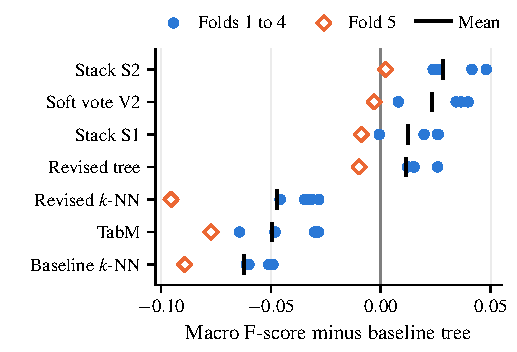
\includegraphics[width=3.45in]{figures/paired_differences.pdf}
    \caption{Outer-fold differences in macro F-score from the baseline tree}
    \label{fig:paired}
\end{figure}

The three measures ranked the models differently. The revised tree had the highest balanced accuracy but the lowest accuracy. Recovering more minority-class observations therefore came with more errors on frequent classes. TabM had the highest accuracy of the base learners but a lower macro F-score than either tree. Accurate classification of frequent classes did not compensate for weak rare-class recovery under macro averaging.

Re-tuning raised the mean macro F-score of both earlier models, with gains on four folds and no significant difference. Fold five gave the smallest S2 gain over the baseline tree. The baseline tree of fold five already used balanced weights, so the fold compared S2 with a stronger minority-sensitive baseline. Other tree settings also differed, preventing isolation of weighting alone.

Stack S1 scored within 0.001 of the revised tree, so the revised \knn{} added almost nothing to the revised tree. Adding TabM raised S2 above S1 on every fold. The raw corrected test was significant, but the Holm-adjusted test was not. The improvement therefore supported further study of TabM as a complementary learner, without a family-level significance claim.

\subsection{Inductive Bias and Class-Specific Performance}
Table~\ref{tab:perclass} shows why the aggregate rankings differed. The baseline tree exceeded baseline \knn{} on eight classes, with the largest advantages on Worms and Shellcode. A tree selects different features in different branches and forms conjunctions of threshold and category tests. Nearest neighbour classification instead applies one distance rule across all encoded features \cite{breiman1984,hastie2009}. Uninformative coordinates and overlapping classes therefore enter every neighbourhood, even where a small feature subset identifies a useful rule. Table~\ref{tab:pr} gives the precision and recall behind the F-scores of four classes.

\begin{table*}[!t]
    \caption{Pooled outer-test F-score of each class}
    \label{tab:perclass}
    \centering\footnotesize
    \begin{tabular}{@{}lcccccccc@{}}
        \toprule
        Class          & Baseline tree & Baseline \knn  & Revised tree   & Revised \knn & TabM           & Stack S1 & Stack S2       & Soft vote V2 \\
        \midrule
        Normal         & 0.909         & 0.900          & 0.856          & 0.904        & 0.918          & 0.917    & \textbf{0.922} & 0.916 \\
        Reconnaissance & 0.831         & 0.713          & 0.825          & 0.757        & 0.832          & 0.835    & \textbf{0.840} & 0.832 \\
        Backdoor       & 0.152         & 0.095          & 0.160          & 0.106        & 0.160          & 0.166    & 0.178          & \textbf{0.233} \\
        DoS            & 0.311         & 0.403          & \textbf{0.472} & 0.419        & 0.102          & 0.303    & 0.309          & 0.433 \\
        Exploits       & 0.716         & 0.683          & 0.645          & 0.697        & \textbf{0.738} & 0.729    & 0.738          & 0.719 \\
        Analysis       & 0.104         & \textbf{0.155} & 0.155          & 0.109        & 0.061          & 0.109    & 0.104          & 0.138 \\
        Fuzzers        & 0.606         & 0.552          & 0.616          & 0.563        & 0.597          & 0.617    & 0.631          & \textbf{0.650} \\
        Worms          & 0.598         & 0.288          & 0.561          & 0.275        & 0.260          & 0.580    & \textbf{0.661} & 0.440 \\
        Shellcode      & 0.615         & 0.349          & 0.582          & 0.476        & 0.602          & 0.633    & \textbf{0.660} & 0.631 \\
        Generic        & 0.987         & 0.985          & 0.987          & 0.986        & 0.988          & 0.988    & \textbf{0.989} & 0.988 \\
        \midrule
        Macro average  & 0.583         & 0.512          & 0.586          & 0.529        & 0.526          & 0.588    & \textbf{0.603} & 0.598 \\
        \bottomrule
    \end{tabular}
\end{table*}

\begin{table*}[!t]
    \caption{Pooled outer-test precision and recall of four classes}
    \label{tab:pr}
    \centering\footnotesize
    \begin{tabular}{@{}lcccccccc@{}}
        \toprule
                      & \multicolumn{2}{c}{Normal} & \multicolumn{2}{c}{Backdoor} & \multicolumn{2}{c}{DoS} & \multicolumn{2}{c}{Worms} \\
        \cmidrule(lr){2-3}\cmidrule(lr){4-5}\cmidrule(lr){6-7}\cmidrule(l){8-9}
        Model         & Precision & Recall & Precision & Recall & Precision & Recall & Precision & Recall \\
        \midrule
        Baseline tree & 0.910 & 0.908 & 0.143 & 0.163 & 0.392 & 0.258 & 0.598 & 0.598 \\
        Baseline \knn & 0.885 & 0.914 & 0.093 & 0.097 & 0.370 & 0.443 & 0.385 & 0.230 \\
        Revised tree  & 0.975 & 0.764 & 0.097 & 0.454 & 0.363 & 0.674 & 0.440 & 0.776 \\
        Revised \knn  & 0.885 & 0.924 & 0.319 & 0.064 & 0.376 & 0.472 & 0.542 & 0.184 \\
        TabM          & 0.895 & 0.943 & 0.739 & 0.090 & 0.676 & 0.055 & 0.794 & 0.155 \\
        Stack S1      & 0.907 & 0.927 & 0.695 & 0.094 & 0.418 & 0.238 & 0.643 & 0.529 \\
        Stack S2      & 0.910 & 0.934 & 0.775 & 0.100 & 0.428 & 0.242 & 0.673 & 0.649 \\
        Soft vote V2  & 0.928 & 0.904 & 0.211 & 0.260 & 0.384 & 0.497 & 0.628 & 0.339 \\
        \bottomrule
    \end{tabular}
\end{table*}

Feature-specific partitioning was a plausible explanation for the stronger rare-class results. The baseline \knn{} recovered fewer than half as many Worms observations as the baseline tree. Worms supplied few neighbours to any query observation, whereas nearby observations of frequent classes competed in every vote. The revised \knn{} selected larger neighbourhoods and recovered still fewer Worms observations, as the bias of a large $k$ predicts. The results supported the tested tree more strongly than the tested distance model for Worms and Shellcode detection. Feature ablations would be needed to identify the responsible predictors.

The tree advantage was not uniform. Baseline \knn{} scored higher on DoS and Analysis, so local similarity retained class information that the selected tree did not exploit equally well. Revising the tree more than doubled DoS recall at slightly lower precision. Balanced weights increased the influence of minority observations during both split selection and leaf prediction. The recall gain matched that mechanism, although other revised settings changed too.

Higher recall did not guarantee a higher F-score. On Worms, the revised tree gained recall but lost precision, and the F-score fell below that of the baseline tree. On Normal, recall fell whereas precision rose. The revised tree therefore issued more minority predictions and required stronger evidence before predicting Normal. These trade-offs explained the rise in balanced accuracy and the fall in accuracy. The precision losses also explained why balanced weighting did not improve every minority F-score.

TabM showed the opposite imbalance. On DoS and Worms, TabM had the highest precision of all models but recovered fewer than one in six observations of either class. The network therefore made selective predictions for these attacks and missed most of the observations. The unweighted cross-entropy gave frequent labels more influence over the total training objective. Shared neural weights coupled decisions across the feature space, whereas tree predictions used separate leaf proportions. These mechanisms were consistent with strong majority classification and weak minority recovery.

Grinsztajn \emph{et al.} linked neural-network difficulties on tabular data to irregular target functions and uninformative features \cite{grinsztajn2022}. The tree--TabM comparison was consistent with that account, but did not test smoothness or feature relevance directly. TabM also scored well on Exploits and Reconnaissance, so the result did not show a general failure to learn the supplied traffic attributes.

Figure~\ref{fig:confusion} compares the baseline tree and S2. S2 recognised more Exploits observations than the tree but also assigned more DoS and Backdoor observations to Exploits. The stack therefore did not resolve the main confusion among these classes. Exploits observations outnumbered DoS observations by 2.7 to one. Of the other observations in conflicting groups that contained DoS observations, 64\% belonged to Exploits. A plausible mechanism is that a meta-learner fitted by likelihood assigns observations that resemble both classes to the more frequent label. The largest S2 F-score gains over the tree were on Worms and Shellcode, the two smallest classes. Macro averaging gave those gains the same influence as gains of equal size on Normal.

\begin{figure*}[!t]
    \centering
    \subfloat[Baseline tree]{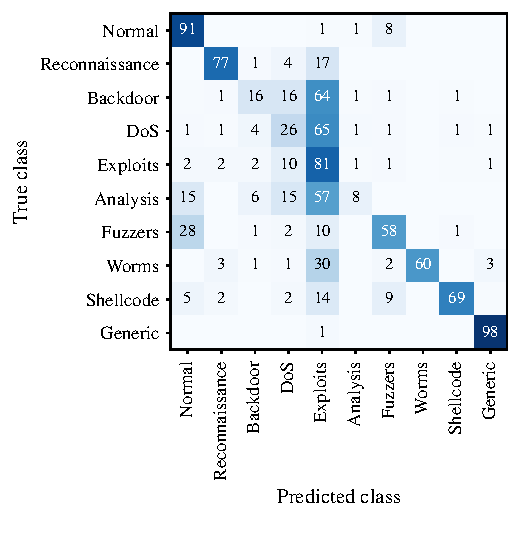
\includegraphics[width=3.45in]{figures/confusion_tree.pdf}}\hfill
    \subfloat[Stack S2]{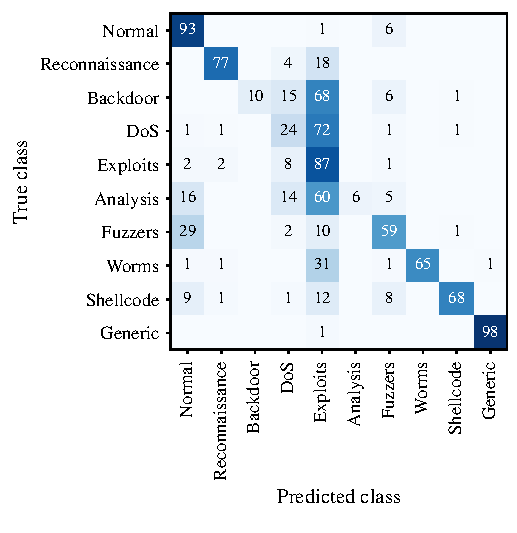
\includegraphics[width=3.45in]{figures/confusion_S2.pdf}}
    \caption{Row-normalised confusion matrices of the pooled outer-test predictions in percent}
    \label{fig:confusion}
\end{figure*}

For Q9, the soft vote had the highest Backdoor F-score of all models and exceeded every one of the three base learners. The revised tree alone remained best on DoS. On Backdoor, the revised tree recovered many observations with low precision, whereas TabM recovered few observations with high precision. Averaging these assignments with the \knn{} probabilities gave V2 a higher Backdoor F-score than any member. The Backdoor gain therefore involved the combination itself, whereas a weighting-only contribution was not measured.

Analysis remained difficult for every model, and no model reached an F-score of 0.16. Most Analysis observations lay in conflicting groups, so class identity was frequently ambiguous from the supplied inputs. The experiment did not separate that ambiguity from model or tuning limitations. The class-specific results contradicted a uniform ensemble advantage.

\subsection{Neural Ensemble Tuning}
Figure~\ref{fig:size} addresses Q1. The ensemble score rose with the number of members, whereas the mean score of a single member stayed flat. Combining outputs therefore improved the prediction without improving the average member, consistent with averaging partly different errors \cite{dietterich2000}. About 60\% of the observed gain arrived by eight members, in line with the Q1 prediction.

\begin{figure}[!t]
    \centering
    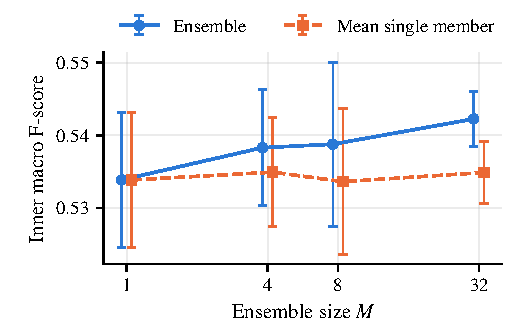
\includegraphics[width=3.45in]{figures/tabm_ensemble_size.pdf}
    \caption{Inner macro F-score against ensemble size, with standard deviations over five outer folds}
    \label{fig:size}
\end{figure}

The smaller standard deviation at 32 members described variation across outer-fold tuning scores and did not establish a reduced training-seed variance. The 32-member point was also selected from 24 capacity candidates, whereas smaller ensembles were follow-ups at the selected capacity. Capacity selection therefore made the estimated size effect optimistic.

Balanced weights lowered the inner macro F-score in Table~\ref{tab:classweights}. The Worms and Shellcode F-scores fell most, refuting Q2. Equalising the total class weight did not equalise uncertainty. An inner fit contained only about 93 Worms observations, and each Worms observation received roughly 148 times the unit loss weight, against 0.28 for Normal. Repeated gradients from a small set of rare observations consequently had much greater influence.

\begin{table}[!t]
    \caption{Inner F-scores of TabM without and with balanced class weights}
    \label{tab:classweights}
    \centering\footnotesize
    \begin{tabular}{@{}lccc@{}}
        \toprule
        Class          & No weights & Balanced weights & Change     \\
        \midrule
        Normal         & 0.914      & 0.847            & $-0.067$   \\
        Reconnaissance & 0.827      & 0.818            & $-0.008$   \\
        Backdoor       & 0.140      & 0.162            & $+0.022$   \\
        DoS            & 0.361      & 0.468            & $+0.107$   \\
        Exploits       & 0.716      & 0.596            & $-0.120$   \\
        Analysis       & 0.067      & 0.170            & $+0.103$   \\
        Fuzzers        & 0.578      & 0.604            & $+0.026$   \\
        Worms          & 0.257      & 0.093            & $-0.164$   \\
        Shellcode      & 0.576      & 0.413            & $-0.163$   \\
        Generic        & 0.986      & 0.986            & $-0.000$   \\
        \midrule
        Macro average  & 0.542      & 0.516            & $-0.027$   \\
        \bottomrule
    \end{tabular}
\end{table}

A plausible explanation was that weighting increased rare-class predictions beyond the precision--recall balance favoured by macro F-score. Tuning did not record class-wise precision, so that mechanism remained unverified for TabM. The tree results demonstrated the relevant trade-off directly, with higher rare-class recall accompanied by lower precision. Weighting acts differently on neural gradients and on tree partitions, a possible reason that the weighting choice did not transfer between model families.

Distinct minibatches lowered the inner score on every fold, by 0.009 on average, and lowered the mean member score from 0.535 to 0.528. Q3 therefore did not support an advantage from separate shuffles. Every member still saw every observation each epoch, so this experiment was not bootstrap bagging. Separate shuffles changed the observations contributing to a shared-weight update as well as the similarity between members. The weaker members indicated that additional batch diversity did not offset the changed optimisation.

Table~\ref{tab:capacity} addresses Q4. Wider and deeper networks scored better on average, consistent with additional capacity for interactions among traffic attributes. No dropout scored highest, and stronger dropout delayed the best epoch. Early stopping and weight sharing already constrained fitting, making extra dropout a plausible source of unnecessary restriction \cite{goodfellow2016,gorishniy2025}. The experiment did not isolate the regularisation mechanisms.

\begin{table}[!t]
    \caption{Inner macro F-score and best epoch of TabM by capacity level}
    \label{tab:capacity}
    \centering\footnotesize
    \begin{tabular}{@{}llcc@{}}
        \toprule
        Factor        & Level              & Inner macro F-score & Best epoch \\
        \midrule
        Width         & 256                & 0.524               & 21.7       \\
                      & 512                & 0.531               & 17.2       \\
        Depth         & 2                  & 0.526               & 19.0       \\
                      & 3                  & 0.530               & 19.8       \\
        Dropout       & 0                  & 0.533               & 16.9       \\
                      & 0.1                & 0.527               & 18.0       \\
                      & 0.2                & 0.522               & 23.4       \\
        Learning rate & $10^{-3}$          & 0.526               & 21.4       \\
                      & $2\times10^{-3}$   & 0.530               & 17.4       \\
        \bottomrule
    \end{tabular}
\end{table}

Capacity effects were small relative to the gap between TabM and the best stack. No tested factor changed the mean inner score by more than 0.012. Increasing capacity within the grid therefore did not remove the model-selection and minority-class trade-offs. The result applied only to the tested widths and depths.

The first-run TabM had reached a macro F-score of 0.549 and a DoS F-score of 0.409, both above the final values. The final protocol trained without validation checkpoint selection. A fold-one seed diagnostic found low DoS recall before seed averaging, so averaging did not explain the failure. Removal of checkpoint selection remained a plausible explanation, because validation macro F-score rewards recovery of small classes even when the training likelihood favours frequent labels. The changed tuning, configurations and training partitions prevented attribution to the epoch rule alone.

\subsection{Stacking and Complementary Predictions}
S2 exceeded soft vote V2 by the smallest mean difference of the 11 paired comparisons in Table~\ref{tab:overall}. Q5 therefore did not establish an advantage from learning the combination. Equal-weight averaging already combined the class-weighted tree with more selective neural predictions. Logistic regression added class-specific and cross-class corrections, but the extra parameters produced little mean improvement over averaging.

The two combinations favoured different outcomes. S2 had the higher accuracy, whereas V2 had the higher balanced accuracy. S2 consequently made fewer total mistakes but recovered fewer observations of each class on average. Per class, S2 scored far higher than V2 on Worms but lower on Backdoor, DoS, Analysis and Fuzzers. Averaged over the other nine classes, the pooled F-scores of V2 exceeded those of S2 by 0.019. The S2 advantage therefore rested on one class with 34 or 35 observations in each test fold. The fitted combination changed the balance separately for each class, whereas V2 retained the minority-class probabilities of the revised tree through a fixed equal-weight average.

Table~\ref{tab:diversity} supports the interpretation of Q6. TabM and the revised tree had the lowest error correlation and the fewest observations misclassified by both learners. TabM therefore frequently supplied a correct prediction where the revised tree failed, despite a lower standalone macro F-score. Lower error correlation was a useful diagnostic of complementarity, but did not isolate the cause of the stack gain \cite{kuncheva2003}.

\begin{table}[!t]
    \caption{Diversity of base-learner pairs on the outer-test folds}
    \label{tab:diversity}
    \centering\footnotesize
    \setlength{\tabcolsep}{4pt}
    \begin{tabular}{@{}lccc@{}}
        \toprule
        Pair                       & Error correlation & Disagreement (\%) & Both wrong (\%) \\
        \midrule
        \knn{} and tree            & 0.460             & 23.8              & 12.5            \\
        \knn{} and TabM            & 0.565             & 16.3              & 12.0            \\
        Tree and TabM              & 0.307             & 28.5              & 9.2             \\
        \bottomrule
    \end{tabular}
\end{table}

Revised-tree sensitivity and TabM selectivity provided a plausible source of the S2 gain over S1. The tree--TabM error correlation differed from the first-run value of 0.605, but several training choices changed simultaneously. Diversity therefore depended on the evaluated configurations, rather than following from model names alone.

Figure~\ref{fig:coefficients} gives standardised own-class coefficients for Q7. TabM had the largest value on eight classes, with the tree largest on Worms and Shellcode. The \knn{} value exceeded the tree value on DoS, but not on Analysis. The predicted ordering was therefore mostly absent.

\begin{figure}[!t]
    \centering
    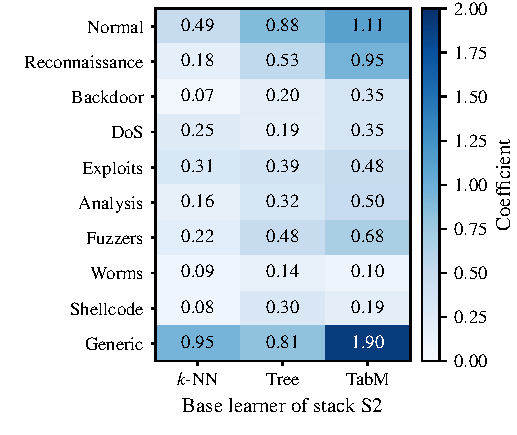
\includegraphics[width=3.45in]{figures/meta_coefficients.pdf}
    \caption{Own-class coefficients of the stack meta-learner averaged over five outer folds}
    \label{fig:coefficients}
\end{figure}

These coefficients described one contribution to a class score. All base probabilities and competing class scores entered the final decision, and each probability block summed to one. A large coefficient did not establish that a learner dominated predictions. TabM supplied graded DoS probabilities even when DoS was not the largest output. Stacking retained probability variation that predicted labels alone would discard.

Table~\ref{tab:representation} addresses Q8 with the best inner score of each representation, averaged over the outer folds. Probabilities scored highest for both stacks. The result supported the value of confidence information, in agreement with Ting and Witten \cite{ting1999}. Log-probabilities scored below probabilities for both stacks. Of the revised \knn{} probabilities, 82\% were zero, and 58\% of observations assigned probability one to a class. The logarithm mapped zeros to about $-9.2$, magnifying differences among these sparse estimates. That transformation did not improve the tested linear meta-learner, although probability calibration was not measured.

\begin{table}[!t]
    \caption{Best inner macro F-score of each meta-feature representation}
    \label{tab:representation}
    \centering\footnotesize
    \begin{tabular}{@{}lcc@{}}
        \toprule
        Representation    & Stack S1          & Stack S2          \\
        \midrule
        Probabilities     & $0.578 \pm 0.006$ & $0.590 \pm 0.005$ \\
        Log-probabilities & $0.561 \pm 0.005$ & $0.577 \pm 0.004$ \\
        One-hot labels    & $0.567 \pm 0.010$ & $0.559 \pm 0.009$ \\
        \bottomrule
    \end{tabular}
\end{table}

\subsection{Computational Cost}
Table~\ref{tab:cost} separates tuning from the three inner refits and the outer-training refit. Each TabM refit included five seeds, so four refits represented 20 trained TabMs. The revised \knn{} and TabM searches shared a GPU, so the recorded durations should not be added to estimate elapsed runtime. Each of the two searches alone took more than 200 times as long per outer fold as the four baseline tree fits.

\begin{table}[!t]
    \caption{Computing time for each outer fold in seconds}
    \label{tab:cost}
    \centering\footnotesize
    \begin{tabular}{@{}llrr@{}}
        \toprule
        Model                 & Device & Tuning   & Four final fits \\
        \midrule
        Baseline tree         & CPU    & --       & 19              \\
        Baseline \knn         & CPU    & --       & 676             \\
        Revised tree          & CPU    & 185      & 16              \\
        Revised \knn          & GPU    & 4\,617   & 216             \\
        TabM                  & GPU    & 4\,977   & 405             \\
        Meta-learner of S2    & CPU    & 64       & --              \\
        \bottomrule
    \end{tabular}
\end{table}

The stack therefore exchanged substantially greater fitting and selection cost for a mean macro F-score gain of 0.028. A single tree remained attractive when retraining cost mattered. S2 would be justified by the measured class-specific gains only if the application valued those gains enough to support the extra computation. Inference latency was not measured.

\subsection{Limitations}
The protocol changed after the first outer-test results were known. The final scores therefore described an exploratory comparison on reused test folds, even though outer-test observations remained outside final-run fitting. Five dependent fold differences also gave low power. Neither S2 against the baseline tree nor S2 against S1 was significant after adjustment across the 11 comparisons. Repeated grouped evaluation under a fixed protocol would test whether the gains persisted.

Inner scores included checkpoint-selection optimism and upstream dependence in meta-validation. The ensemble-size comparison additionally favoured the capacity-selected 32-member reference. These limitations constrained causal interpretation of tuning effects. Independent checkpoint validation and rebuilding base predictions within meta-training partitions would provide cleaner comparisons.

The study covered one traffic dataset, a finite neural-capacity grid and a linear meta-learner. Robust scaling also left \texttt{response\_body\_len} unscaled, so response size dominated the selected \knn{} distances between observations with a response body. A logarithmic transformation before scaling was not tested. Differences in weighting, tuning budgets and final training prevented attribution of score gaps to inductive bias alone. The proposed mechanisms were supported by observed error patterns, but required controlled ablations to separate model structure from training choices.

\section{Conclusions}
The study compared neural network ensembles and stacking with $k$-nearest neighbours (\knn) and a decision tree on network intrusion classification. TabM combined multilayer perceptrons (MLPs) through shared weights. Stacking combined the probabilities of TabM and the re-tuned earlier models. Nine questions guided tuning and class-specific analysis on the earlier five grouped outer folds.

The three-learner stack had the highest mean macro F-score and exceeded the earlier tree on every fold, but the gain was not statistically significant. The tree recovered Worms and Shellcode more effectively than \knn{} under the tested settings. Feature-specific partitioning provided a plausible explanation for that advantage over a single distance rule. Balanced weighting increased tree recall but also introduced false positive attack predictions. TabM was more selective on rare classes and more accurate on frequent classes.

TabM alone scored below both trees but improved the stack on every fold. The low error correlation with the revised tree supported the usefulness of complementary predictions. Learned stacking did not establish an advantage over equal-weight averaging, and the small lead of the stack over the soft vote rested on Worms alone. The soft vote improved Backdoor F-score beyond every base learner, whereas the revised tree remained best on denial of service (DoS). No ensemble improved every class.

Increasing TabM members gave a small inner-score gain. Balanced weights, separate minibatches and dropout lowered the tested tuning scores. The fall in final DoS recall was already present before seed averaging, but the experiment did not isolate the responsible training change. These findings applied to the selected configurations and the protocol revised after the first test results.

Further work was needed on repeated grouped evaluation under a fixed protocol and on matched ablations of weighting and checkpoint selection. Class-specific thresholds selected on independent inner validation would test the minority-recall trade-off directly. Evaluating the already tested class-weighted meta-learners under an explicit recall or cost criterion would also distinguish the application objective from unweighted likelihood.

\appendices
\section{Acronyms}
\footnotesize
\begin{tabular}{@{}l>{\raggedright\arraybackslash}p{6.2cm}@{}}
    \toprule
    Acronym & Meaning                                                \\
    \midrule
    Adam    & adaptive moment estimation                             \\
    AdamW   & Adam with decoupled weight decay                       \\
    CPU     & central processing unit                                \\
    DoS     & denial of service                                      \\
    GPU     & graphics processing unit                               \\
    \knn    & $k$-nearest neighbours                                 \\
    L-BFGS  & limited-memory Broyden--Fletcher--Goldfarb--Shanno     \\
    MLP     & multilayer perceptron                                  \\
    ReLU    & rectified linear unit                                  \\
    UNSW    & University of New South Wales                          \\
    \bottomrule
\end{tabular}

\section{Symbols}
\footnotesize
\begin{tabular}{@{}ll@{}}
    \toprule
    Symbol                         & Meaning                                          \\
    \midrule
    $A$                            & accuracy                                         \\
    $\mathbf{a}$, $\mathbf{a}'$    & input and output of a hidden layer               \\
    $\mathbf{a}_h$                 & input of member $h$ to a BatchEnsemble layer     \\
    $\mathbf{b}$                   & bias vector of a hidden layer                    \\
    $\mathbf{b}_h$                 & bias vector of member $h$                        \\
    $C$                            & inverse regularisation strength                  \\
    $D_v$                          & difference in macro F-score on fold $v$          \\
    $\bar{D}$                      & mean of the fold differences                     \\
    $d$                            & distance function                                \\
    $e$                            & total sample-weighted leaf impurity of a tree       \\
    $F_l$                          & F-score of class $l$                             \\
    $\bar{F}$                      & macro F-score                                    \\
    $G$                            & Gini impurity                                    \\
    $H$                            & entropy                                          \\
    $h$                            & member index                                     \\
    $i$                            & observation index                                        \\
    $j$                            & feature index                                    \\
    $K$                            & number of classes                                \\
    $k$                            & number of neighbours                             \\
    $l$, $l'$                      & class indices                                    \\
    $\mathcal{L}$                  & TabM loss of one observation                             \\
    $M$                            & number of TabM members                           \\
    $m$                            & number of features                               \\
    $N_k$                          & index set of the $k$ nearest neighbours          \\
    $n$                            & number of training observations                          \\
    $n_l$                          & number of training observations of class $l$             \\
    $\mathbf{o}_h$                 & output of member $h$ of a BatchEnsemble layer    \\
    $P_l$                          & precision of class $l$                           \\
    $p$                            & probability value of a test                      \\
    $Q$                            & impurity of a node                               \\
    $\Delta Q$                     & impurity decrease of a test                      \\
    $q$                            & order of the Minkowski distance                  \\
    $R_l$                          & recall of class $l$                              \\
    $\bar{R}$                      & balanced accuracy                                \\
    $\mathbf{r}_h$, $\mathbf{s}_h$ & input and output scaling vectors of member $h$   \\
    $S_t$                          & training observations at node $t$                        \\
    $S_L$, $S_R$                   & training observations of the left and right child        \\
    $T$                            & subtree of a pruned tree                         \\
    $|T|$                          & number of leaves of $T$                          \\
    $t$                            & tree node                                        \\
    $t_L$, $t_R$                   & left and right child nodes                       \\
    $V$                            & number of cross-validation folds                 \\
    $v$                            & fold index                                       \\
    $\mathbf{W}$                   & weight matrix of a layer                         \\
    $\mathbf{W}_h$                 & effective weight matrix of member $h$            \\
    $w_i$                          & vote weight of neighbour $i$                     \\
    $\mathbf{x}$, $\mathbf{x}'$    & predictor vectors                                \\
    $x_j$                          & feature $j$ of a predictor vector                \\
    $y$, $\hat{y}$                 & true and predicted class                         \\
    $\mathbf{z}$                   & meta-feature vector                              \\
    $\alpha$                       & pruning penalty for each leaf                    \\
    $\bm{\beta}_l$, $\beta_{l,0}$  & meta-learner coefficients and intercept          \\
    $\delta$                       & Kronecker delta                                  \\
    $\theta$                       & split threshold                                  \\
    $\pi_l(t)$                     & proportion of class $l$ at node $t$              \\
    $\hat{\pi}_l$                  & estimated probability of class $l$               \\
    $\hat{\pi}_{h,l}$              & probability of class $l$ from member $h$         \\
    $\hat{\sigma}^2$               & sample variance of the fold differences          \\
    $\tau$                         & corrected resampled t statistic                  \\
    $\omega_l$                     & weight of class $l$                              \\
    $\odot$                        & elementwise product                              \\
    \bottomrule
\end{tabular}

\bibliographystyle{IEEEtranS}
\bibliography{references}
\end{document}
